% $Header$

\documentclass{beamer}

% This file is a solution template for:

% - Talk at a conference/colloquium.
% - Talk length is about 20min.
% - Style is ornate.



% Copyright 2004 by Till Tantau <tantau@users.sourceforge.net>.
%
% In principle, this file can be redistributed and/or modified under
% the terms of the GNU Public License, version 2.
%
% However, this file is supposed to be a template to be modified
% for your own needs. For this reason, if you use this file as a
% template and not specifically distribute it as part of a another
% package/program, I grant the extra permission to freely copy and
% modify this file as you see fit and even to delete this copyright
% notice. 


\mode<presentation>
{
  \usetheme{Warsaw}
  % or ...

  \setbeamercovered{transparent}
  % or whatever (possibly just delete it)
}


\usepackage[english]{babel}
% or whatever

\usepackage[utf8]{inputenc}
% or whatever

\usepackage{tikz}
\usetikzlibrary{arrows, shapes, snakes}

\usepackage{times}
\usepackage[T1]{fontenc}
% Or whatever. Note that the encoding and the font should match. If T1
% does not look nice, try deleting the line with the fontenc.

%\newtheorem{definition}{Definition}

\title% (optional, use only with long paper titles)
{Consensus and replication}

\subtitle
{From impossibility to production}

\author[Alexander Kharitonov]{Alexander Kharitonov \\ \texttt{skywalker@yandex-team.ru}}
\date{Yandex science seminar, 22 Mar 2012}

%\author[Author, Another] % (optional, use only with lots of authors)
%{F.~Author\inst{1} \and S.~Another\inst{2}}
% - Give the names in the same order as the appear in the paper.
% - Use the \inst{?} command only if the authors have different
%   affiliation.
%\institute[Yandex]
%{
%    Yandex LLC
%}

%\institute[Universities of Somewhere and Elsewhere] % (optional, but mostly needed)
%{
%  \inst{1}%
%  Department of Computer Science\\
%  University of Somewhere
%  \and
%  \inst{2}%
%  Department of Theoretical Philosophy\\
%  University of Elsewhere}
% - Use the \inst command only if there are several affiliations.
% - Keep it simple, no one is interested in your street address.

%\date[CFP 2003] % (optional, should be abbreviation of conference name)
%{Conference on Fabulous Presentations, 2003}
% - Either use conference name or its abbreviation.
% - Not really informative to the audience, more for people (including
%   yourself) who are reading the slides online

\subject{Distributed systems}
% This is only inserted into the PDF information catalog. Can be left
% out. 



% If you have a file called "university-logo-filename.xxx", where xxx
% is a graphic format that can be processed by latex or pdflatex,
% resp., then you can add a logo as follows:

% \pgfdeclareimage[height=0.5cm]{university-logo}{university-logo-filename}
% \logo{\pgfuseimage{university-logo}}



% Delete this, if you do not want the table of contents to pop up at
% the beginning of each subsection:
\AtBeginSubsection[]
{
  \begin{frame}<beamer>{Outline}
    \tableofcontents[currentsection,currentsubsection]
  \end{frame}
}


% If you wish to uncover everything in a step-wise fashion, uncomment
% the following command: 

%\beamerdefaultoverlayspecification{<+->}


\begin{document}

\begin{frame}
  \titlepage
\end{frame}

\begin{frame}{Outline}
  \tableofcontents
  % You might wish to add the option [pausesections]
\end{frame}


% Structuring a talk is a difficult task and the following structure
% may not be suitable. Here are some rules that apply for this
% solution: 

% - Exactly two or three sections (other than the summary).
% - At *most* three subsections per section.
% - Talk about 30s to 2min per frame. So there should be between about
%   15 and 30 frames, all told.

% - A conference audience is likely to know very little of what you
%   are going to talk about. So *simplify*!
% - In a 20min talk, getting the main ideas across is hard
%   enough. Leave out details, even if it means being less precise than
%   you think necessary.
% - If you omit details that are vital to the proof/implementation,
%   just say so once. Everybody will be happy with that.

\section{Motivation}
\subsection{Example: leader election}

\begin{frame}
  Consider a classic semi-synchronous master-slave replication scheme with quorum writes.
  \begin{figure}[!h]
  \centering
  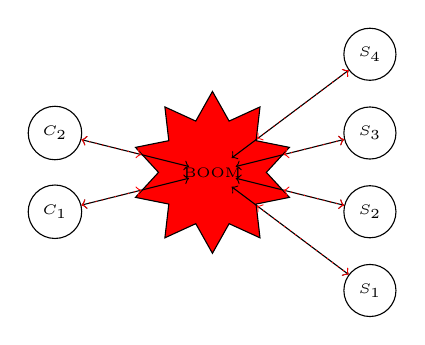
\begin{tikzpicture}
    \tikzstyle{every node} = [draw]
    \node (c1) [circle] at (0, 1) {\tiny $C_1$};
    \node (c2) [circle] at (0, 2) {\tiny $C_2$};
    \invisible<2>{\node (m)  [circle] at (2, 1.5) {\tiny $M$};}
    \invisible<1>{\node (fm) [star, star points=10, fill=red] at (2, 1.5) {\tiny BOOM};}
    \node (s1) [circle] at (4, 0) {\tiny $S_1$};
    \node (s2) [circle] at (4, 1) {\tiny $S_2$};
    \node (s3) [circle] at (4, 2) {\tiny $S_3$};
    \node (s4) [circle] at (4, 3) {\tiny $S_4$};
    \invisible<2>{
      \foreach \from/\to in {c1/m, c2/m}
        \draw [<->] (\from) -- (\to);
      \foreach \from/\to in {m/s1, m/s2, m/s3, m/s4}
        \draw [<->] (\from) -- (\to);
    }
    \invisible<1>{
      \foreach \from/\to in {c1/fm, c2/fm}
        \draw [red, dotted, <->] (\from) -- (\to);
      \foreach \from/\to in {fm/s1, fm/s2, fm/s3, fm/s4}
        \draw [red, dotted, <->] (\from) -- (\to);
    }
  \end{tikzpicture}
  \end{figure}
  \visible<2>{ As we all know, manual master failover sucks. }
\end{frame}

\begin{frame}{Master election}
  \begin{itemize}
    \item  To maintain data consistency in this setting, the master election protocol \alert{must} provide the following guarantees:
      \begin{itemize}
        \item Only a single master is chosen.
        \item A participant never learns that a process $M$ is chosen to be master unless it is actually chosen.
      \end{itemize}
    \item It also makes sense to require that only an active process can be chosen (e.g. not to elect a dead replica that takes no part in the protocol).
    \item The protocol must also be fault-tolerant in some sense (remember the BOOM?).
    \item This protocol is essentially \alert{consensus} on the identity of the master.
  \end{itemize}
\end{frame}

\subsection{Consensus}
\begin{frame}{Consensus}
  \begin{itemize}
    \item Consider a collection of processes that can propose values. A \alert{consensus} algorithm ensures that a single value among the proposed ones is chosen and the processes are then able to learn the chosen value.
    \item The \alert{safety} properties of consensus are:
      \begin{itemize}
        \item Only a value that has been proposed has been chosen.
        \item Only a single value is chosen.
        \item A process never learns that a value has been chosen unless it actually has been.
      \end{itemize}
    \item The liveness property is that if enough processes stay alive, then eventually a value is chosen and all nonfaulty processes eventually learn it.
  \end{itemize}
\end{frame}

\begin{frame}{Process roles}
  \begin{itemize}
    \item Proposers propose values.
    \item Acceptors accept proposals and choose the consensus value.
    \item Learners learn the chosen value.
  \end{itemize}
\end{frame}

\begin{frame}{A few words on the model}
  We assume the \alert{asynchronous} model with \alert{non-Byzantine} faults. It means that:
  \begin{itemize}
    \item Processes operate at arbitrary speeds, have no shared clocks and no bound on clock drift. They may fail by stopping and restart afterwards. Each process has stable storage which survives failures.
    \item Processes communicate by sending messages. Messages can take arbitrarily long to be delivered, can be duplicated, reordered and lost, but \alert{cannot be corrupted}.
  \end{itemize}
\end{frame}

\begin{frame}{So let's try to build a consensus algorithm!}
  A na\"ive algorithm would use a single distinguished acceptor which chooses the first proposal it receives. It is safe, but it does not tolerate the failure of that single acceptor.
  \begin{figure}[!h]
  \centering
  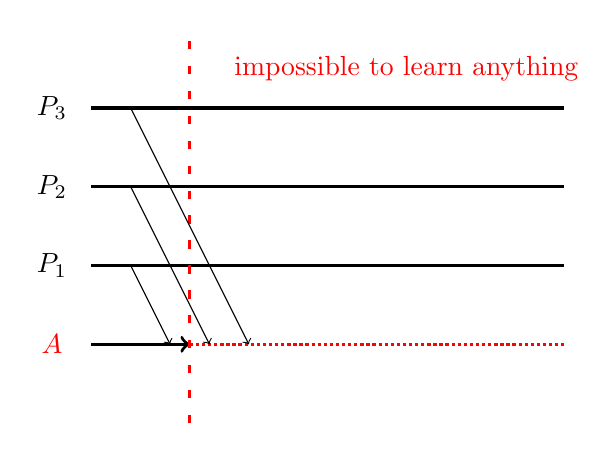
\begin{tikzpicture}
%    \tikzstyle{every node} = [draw]
    \foreach \n in {1, 2, 3} {
      \node at (-0.5, \n) {$P_\n$};
      \draw [very thick] (0, \n) -- (6, \n);
    }
    \node [red] at (-0.5, 0) {$A$};
    \node [red] at (4, 3.5) {impossible to learn anything};
    \draw [very thick, ->] (0, 0) -- (1.25, 0);
    \draw [densely dotted, very thick, red] (1.25, 0) -- (6, 0);
    \draw [loosely dashed, very thick, red] (1.25, -1) -- (1.25, 4);
    \draw [thin, ->] (0.5, 3) -- (2, 0);
    \draw [thin, ->] (0.5, 2) -- (1.5, 0);
    \draw [thin, ->] (0.5, 1) -- (1, 0);
  \end{tikzpicture}
  \end{figure}
\end{frame}

\newtheorem{invariant}[theorem]{Invariant}

\begin{frame}{Okay, let's have many acceptors!}
  \begin{itemize}
    \item Let's say that a value has been chosen when a large enough set of acceptors accepted it.
    \item Large enough -- e.g. a majority.
    \item If an acceptor can accept \alert{at most one value}, then safety is guaranteed, because any two majorities have an element in common!
    \item Without failures and message loss, want to choose a value if there is only \alert{one} proposer and it proposes \alert{one} value. This suggests the following invariant:
  \end{itemize}
  \begin{invariant}[P1]
    A proposer must accept the first value it receives.
  \end{invariant}
\end{frame}

\begin{frame}{Just P1 and the majority rule aren't good enough}
  \begin{figure}[!h]
  \centering
  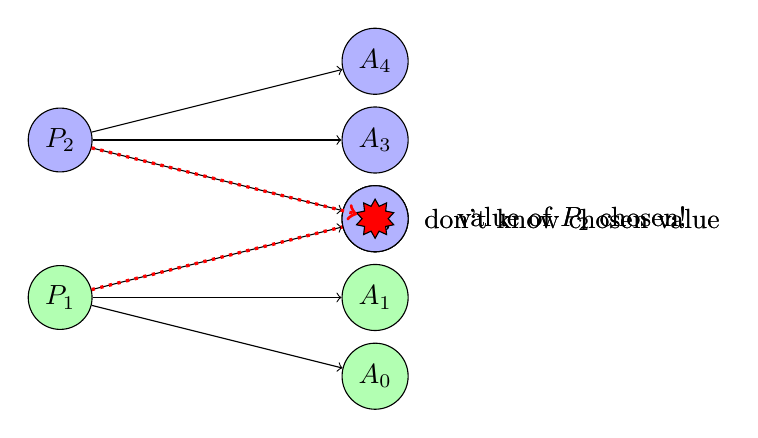
\begin{tikzpicture}
    \tikzstyle{every node} = [shape=circle]
    \node (p1) [draw, fill=green!30] at (0, 1) {$P_1$};
    \node (p2) [draw, fill=blue!30] at (0, 3) {$P_2$};
    \foreach \n in {0, 1} {
      \node (a\n) [draw, fill=green!30] at (4, \n) {$A_\n$};
      \draw [->] (p1) -- (a\n);
    }
    \foreach \n in {3, 4} {
      \node (a\n) [draw, fill=blue!30] at (4, \n) {$A_\n$};
      \draw [->] (p2) -- (a\n);
    }
    \visible<2>{
        \node (A) [draw, fill=green!30] at (4, 2) {$A_3$};
        \node at (6.5, 2) {value of $P_1$ chosen!};
        \draw [->] (p1) -- (A);
    }
    \visible<3>{
        \node (A) [draw, star, star points=10, fill=red] at (4, 2) {};
        \node at (6.5, 2) {don't know chosen value};
        \draw [dotted, very thick, ->, red] (p1) -- (A);
    }
    \visible<1,4>{
        \node (A) [draw] at (4, 2) {$A_3$};
    }
    \visible<5>{
        \node (A) [draw, fill=blue!30] at (4, 2) {$A_3$};
        \node at (6.5, 2) {value of $P_2$ chosen!};
        \draw [->] (p2) -- (A);
    }
    \visible<6>{
        \node (A) [draw, star, star points=10, fill=red] at (4, 2) {};
        \node at (6.5, 2) {don't know chosen value};
        \draw [dotted, very thick, ->, red] (p2) -- (A);
    }

  \end{tikzpicture}
  \end{figure}
\end{frame}

\begin{frame}{Multiple proposals}
  To counter this deadlock, we must allow the acceptors to accept more than one proposal.
  \begin{itemize}
    \item A proposal is a pair $(n, v)$ where $n \in \mathbb{N}$ and $v$ is a proposed value. Different proposals must have different numbers.
    \item A value is chosen when a \alert{single proposal with that value} is accepted by a majority of acceptors.
  \end{itemize}
\end{frame}

\begin{frame}{Consistency with multiple proposals}
  We must allow multiple proposals to be chosen to avoid the aforementioned deadlock, but how do we guarantee consistency?
  \begin{invariant}[P2]
    If a proposal with value $v$ is chosen, then every higher-numbered proposal that is chosen has value $v$.
  \end{invariant}
  \begin{itemize}
    \item Consistency now follows from the fact that $\mathbb{N}$ is totally ordered.
    \item How do we enforce $P2$ though?
  \end{itemize}
\end{frame}

\begin{frame}{Consistency of multiple proposals}
  \begin{invariant}[$P2^a$]
    If a proposal with value $v$ is chosen, then every higher-numbered proposal accepted by \alert{any} acceptor has value $v$.
  \end{invariant}
\end{frame}

\begin{frame}{$P2^a$ doesn't play well with $P1$}
  \begin{figure}[!h]
  \centering
  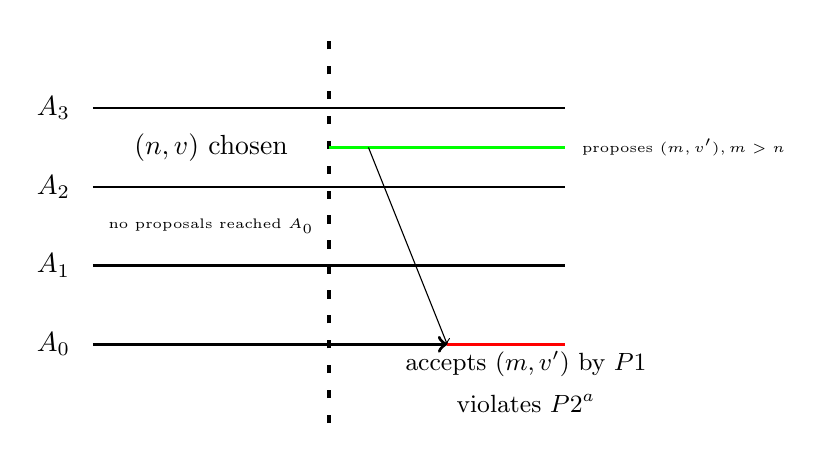
\begin{tikzpicture}
%    \tikzstyle{every node} = [draw]
    \foreach \n in {1, 2, 3} {
      \node at (-0.5, \n) {$A_\n$};
      \draw [thick] (0, \n) -- (6, \n);
    }
    \node at (-0.5, 0) {$A_0$};
    \draw [very thick, ->] (0, 0) -- (4.5, 0);
    \draw [very thick, red] (4.5, 0) -- (6, 0);
    \draw [loosely dashed, very thick] (3, -1) -- (3, 4);
    \node at (1.5, 2.5) {$(n, v)$ chosen};
    \node at (1.5, 1.5) {\tiny no proposals reached $A_0$};

    \draw [thick, green] (3, 2.5) -- (6, 2.5);
    \node at (7.5, 2.5) {\tiny proposes $(m, v'), m > n$};

    \draw [thin, ->] (3.5, 2.5) -- (4.5, 0);
    \node at (5.5, -0.25) {\small accepts $(m, v')$ by $P1$};
    \node at (5.5, -0.75) {\small violates $P2^a$};
  \end{tikzpicture}
  \end{figure}
\end{frame}

\begin{frame}{How do we fix this? By magic.}
  Let's strengthen $P2^a$.

  \begin{invariant}[$P2^b$]
    If a proposal with value $v$ is chosen, then every higher-numbered proposal \alert{issued} by any proposer has value $v$.
  \end{invariant}

  \begin{itemize}
    \item This is actually the correct invariant, but maintaining it is subtle.
    \item No single process knows that a proposal is chosen the moment it is chosen!
    \item How do we extract the maybe-chosen value to issue a proposal?
  \end{itemize}
\end{frame}

\begin{frame}{Maintaining $P2^b$}
  \begin{itemize}
    \item Suppose a proposer wants to issue a proposal numbered $n$.
    \item It asks a majority $Q$ of acceptors for their \alert{highest-numbered accepted proposal} with proposal number \alert{less than $n$}.
    \item If there was some $(m, v), m < n$ that was chosen, then it was chosen by some $Q'$. $Q$ and $Q'$ have an acceptor in common, so the correct value is the value of one of our gathered proposals. How do we find it?
    \item By induction on $P2^b$ all proposals ever issued (and accepted) with numbers in $[m, n)$ have value $v$.
    \item So if we have one proposal from $Q$ in our set (with value $v$), then all higher-numbered also have $v$. Just take the maximum.
  \end{itemize}
\end{frame}

\begin{frame}{Maintaining $P2^b$: a picture}
  \begin{figure}[!h]
  \centering
  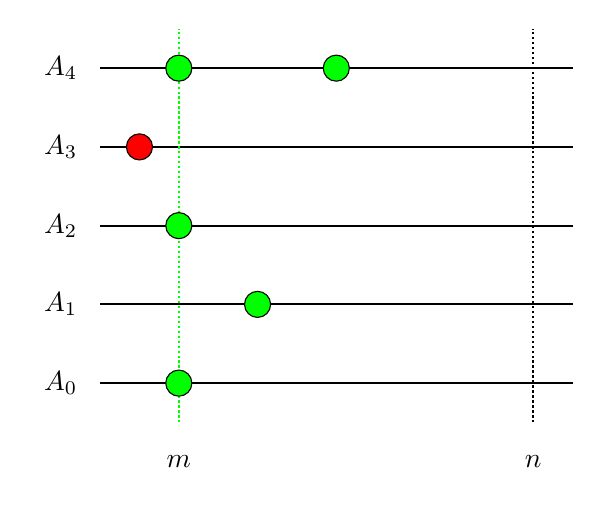
\begin{tikzpicture}
    \tikzstyle{every node} = [shape=circle]
    \foreach \n in {0, 1, 2, 3, 4} {
      \node at (-0.5, \n) {$A_\n$};
      \draw [thick] (0, \n) -- (6, \n);
    }

    \draw [thick, densely dotted, green] (1, -0.5) -- (1, 4.5);
    \node at (1, -1) {$m$};
    \draw [thick, densely dotted] (5.5, -0.5) -- (5.5, 4.5);
    \node at (5.5, -1) {$n$};

    \node [draw, fill=red] at (0.5, 3) {};

    \foreach \n in {0, 2, 4}
      \node [draw, fill=green] at (1, \n) {};

    \node [draw, fill=green] at (2, 1) {};
    \node [draw, fill=green] at (3, 4) {};
  \end{tikzpicture}
  \end{figure}
\end{frame}

\begin{frame}{More on $P2^b$}
  \begin{itemize}
    \item Note that if there is a majority $Q$ that has \alert{no} accepted proposals numbered less than $n$ then this $Q$ certifies that the proposer is free to propose any value in proposal $n$ without compromising $P2^b$.
    \item So, the algorithm for a proposal number $n$ is to collect a majority of highest-numbered accepted proposals having numbers less than $n$, select the highest-numbered and propose its value or propose own value if none... isn't it?
  \end{itemize}
\end{frame}

\begin{frame}{No it isn't!}
  \begin{figure}[!h]
  \centering
  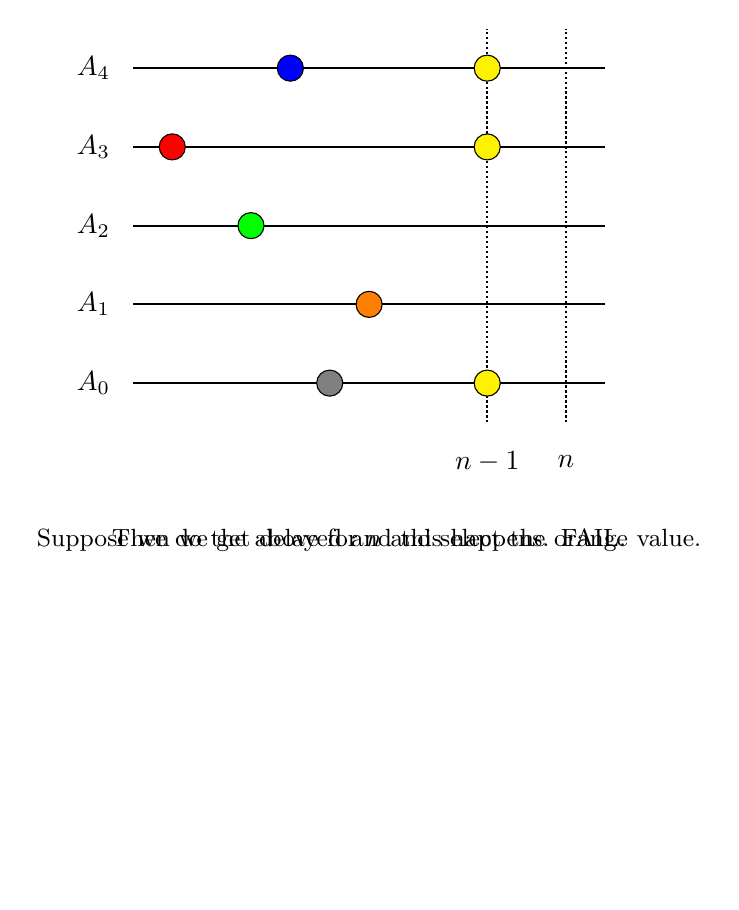
\begin{tikzpicture}
    \tikzstyle{every node} = [shape=circle]
    \foreach \n in {0, 1, 2, 3, 4} {
      \node at (-0.5, \n) {$A_\n$};
      \draw [thick] (0, \n) -- (6, \n);
    }

    \draw [thick, densely dotted] (5.5, -0.5) -- (5.5, 4.5);
    \node at (5.5, -1) {$n$};

    \node [draw, fill=red] at (0.5, 3) {};
    \node [draw, fill=green] at (1.5, 2) {};
    \node [draw, fill=blue] at (2, 4) {};
    \node [draw, fill=gray] at (2.5, 0) {};
    \node [draw, fill=orange] at (3, 1) {};

    \visible<1>{
      \node at (3, -2) {\small Suppose we do the above for $n$ and select the orange value.};
    }
    \visible<2> {
      \node at (3, -2) {\small Then we get delayed and this happens. FAIL.};
      \draw [thick, densely dotted] (4.5, -0.5) -- (4.5, 4.5);
      \node at (4.5, -1) {$n-1$};
      \foreach \n in {0, 3, 4}
        \node [draw, fill=yellow] at (4.5, \n) {};
    }
  \end{tikzpicture}
  \end{figure}
\end{frame}

\begin{frame}{What do we do to uphold $P2^b$?}
  \begin{itemize}
    \item We would be okay if we could gather the accepted less-than-$n$ proposals, calculate the maximum and propose it in one atomic step, but good luck doing that in an asynchronous distributed system.
    \item Instead, when asking the acceptors for their maximal less-than-$n$ accepted proposal, we ask them to \alert{promise} not to accept any proposal numbered less than $n$ after they receive our request.
    \item Now it is easy to see that $P2^b$ always holds and consistency is thus achieved.
    \item We have broken $P1$, though, but we can live with it.
  \end{itemize}
\end{frame}

\begin{frame}{Modifying $P1$}
  \begin{invariant}[$P1^a$]
    An acceptor must accept any proposal it receives if it has not promised not to do so to some proposer.
  \end{invariant}

  Note that while this is weaker than $P1$, it achieves the same purpose. If there is only one proposer and no process and network failures, then nothing will cause the acceptors to make promises harmful to the proposer's progress, so the first proposal will be accepted.
\end{frame}
\end{document}


